\documentclass{article}
\usepackage{amsmath, amssymb, IEEEtrantools}
\usepackage{amsthm}
\usepackage{graphicx}
\usepackage{array}

\title{Representation of Mathematical Expressions in \LaTeX}
\author{Simon Xiang}
\date{\today}
\theoremstyle{definition}
\newtheorem{definition}{Definition}

\begin{document}
\begin{titlepage}
    \begin{center}
        \vspace*{1cm}
 
        \Huge
        \textbf{Experiment 7: Conservation of Momentum}
 
        \vspace{0.5cm}
        \LARGE
        PHYS LAB 1730
 
        \vspace{1.5cm}
 
        \textbf{Simon Xiang}
 
        \vfill
  
        \vspace{0.8cm}
 
        \Large
        Physics Lab Section 518\\
        University of North Texas\\
        \today
 
    \end{center}
\end{titlepage}

\section{Abstract}
The objective of this experiment was to show that momentum is conserved in an isolated system, or that the 
initial momentum of the system is equal to the final momentum of a system after a one-dimensional collision.
Another objective was to see the effect of inelastic versus elastic collisions on the system, and how they conserved or
didn't conserve kinetic energy. 
Our results results ultimately showed that momentum was indeed conserved during collisions, and that 
kinetic energy was conserved relative to whether the collision was elastic or inelastic. The average
percent differences between the initial momentum and final momentum of the system during trials $1$ and $2$ were $15.78\%$
 and $14.74\%$ respectively. This shows that momentum is relatively conserved pre and post collisions, with the error
 being how far the percent values are off from $0\%$, since in an ideal system momemtum is fully conserved. Therefore,
 our results are consistent with the law of conservation of momentum.
\section{Introduction}
The law of conservation of momentum is a crucial law to the study of physics because it shows that no matter what type of collision, inelastic or elastic, momentum is still conserved. In this experiment, 
the objective was to demonstrate the law of conservation of momentum by comparing the momentum of a system before and after a one-dimensional collision.
The significance of this experiment was that one of the most important results in the field of physics was demonstrated experimentally, 
allowing us to verify that it is indeed applicable within the conditions of this experiment.

As a primer, let us precisely define what it means for a particle to have momentum. The momentum $p$ of a particle is defined by 
\begin{equation}
    \vec{p} = m\vec{v},
\end{equation}
where $m$ is a scalar quantity given by the mass of the particle, and $\vec{v}$ is a vector quantity given by the velocity of the particle. 
Since scalar multiplication between a scalar and a vector yields a vector, it is important to note that momentum is defined as a vector, that 
is, it has both magnitude and direction. Before we define the law of conservation of momentum, let us first turn our attention to
the formula for the kinetic energy of an object, given by 
\begin{equation}
    K\!E = \frac{1}{2}m \! \mid \! \vec{v} \! \mid ^2, 
\end{equation}
where $K\!E$ is the kinetic energy of the object, $m$ is the mass of the object (a scalar quantity), and 
$\mid \! \! \vec{v} \! \mid ^2$ denotes the magnitude of the velocity of the object, which is a scalar quantity. It can be seen that
kinetic energy is a scalar quantity since it is the product of two scalar quantities under scalar multiplication. 

Consider the mathematical representation of the law of conservation of momentum, given by 
\begin{equation}
    \vec{p} = \vec{p} \,',
\end{equation}
where $p$ is the momentum of the system before the collision and is defined by 
\begin{equation}
    \vec{p} = m_1 \vec{v_1} + m_2 \vec{v_2},
\end{equation}
where $m_1, m_2$ and $v_1, v_2$ are the masses and velocities before the collision of objects $1$ and $2$ in the isolated system respectively.
Similarly, $p'$ is used to denote the momentum of the system after the collision, and is defined by 
\begin{equation}
    \vec{p} \,' = m_1 \vec{v_1}\,' + m_2 \vec{v_2}\,',
\end{equation}
where $\vec{v_1}\,'$ and $\vec{v_1}\,'$ denote the velocities of objects $1$ and $2$ after the collision respectively. Notice that 
the variables $m_1$ and $m_2$ are the same as the variables $m_1$ and $m_2$ used to define $\vec{p}$. This is because in the case of these particular collisions, 
the mass  of the objects are not changing before and after such aforementioned collision. 

In essence, the law of conservation of momentum states that the momentum of a system before a collision, given by $\vec{p}$,
is the same as the momentum of a system after a collision, given by $\vec{p}\,'$.

\section{Apparatus}
The apparatus used are listed below: 
\begin{itemize}
    \item Air track
    \item Glider (x2)
    \item Rubber band accessory
    \item Wax tube accessory
    \item Nail end accessory 
    \item Photogates 1 and 2.
\end{itemize}
The purpose of the experiment was to determine the law of conservation of momentum through collisions, making the surface upon which
the collisions occured and the objects themselves, the air track and the gliders respectively, quite essential. 
The rubber band accessory was attached to the ends of the track for all trials, and to the ends of the gliders in the case of an elastic collision.
The wax tube accessory was attached to one of the gliders and the nail end accessory attached to the other in the case of an inelastic collision. Finally, 
the photogates were used to record the speed and times of the gliders as they pass through them, and sent such data to the computer system so it could 
calculate the momentum and kinetic energy of the gliders. 
\section{Experimental Procedure}
\begin{enumerate}
    \item Make sure that the air track is level with the ground, and place the photogates on the far ends of the track, about 70 cm away from the edges.
    \item Attach the rubber band accessories to the far ends of the track.
    \item \textbf{Inelastic Collisions:} 
    \begin{enumerate}
    \item Let $\vec{v_1} > 0$ and $\vec{v_2} = 0$ for both trials. For Trial 1, let $m_1 = m_2$, and for Trial 2, let $m_1 > m_2$. Make sure to perform each trial three times for a total of six trials.
    \item Attach the wax tube and nail end accessories to glider 1 and 2 respectively so that the wax tube and nail end accessories face each other. Attach the rubber band accessories to the ends of the gliders that face the ends of the track. 
    \item Pull back glider 1 and release it, and record the values determined by the computer system of the momentum and the kinetic energy of the gliders before and after the collision.
    \end{enumerate}
    \item \textbf{Elastic Collisions:} 
    \begin{enumerate}
    \item Let $\vec{v_1} > 0$ and $\vec{v_2} = 0$ for both trials. For Trial 3, let $m_1 = m_2$, and for Trial 4, let $m_1 > m_2$. Make sure to perform each trial three times for a total of six trials.
    \item Attach the rubber band accessories to both gliders so that they face each other, and attach the flat bumper accessories to the glider such that the flat bumper accessory faces the end of the air track.
    \item Pull back glider 1 and release it, and record the values determined by the computer system of the momentum and the kinetic energy of the gliders before and after the collision.
\end{enumerate}
    \item Using the formula below, calculate the percent difference between the momentum of the system before and after the collision. \begin{equation}
        \text{Percent Difference} = \frac{\mid \!\vec{p} - \vec{p}\,' \!\!\mid}{\frac{\mid \vec{p} + \vec{p}\,' \!\mid}{2}} \cdot 100\%
    \end{equation}
    \item Sum up the percent differences and calculate the average percent difference for momentum per trial.
    \item Using the formula below, calculate the percent difference between the kinetic energy of the system before and after the collision. \begin{equation}
        \text{Percent Difference} = \frac{K\!E - K\!E'}{\frac{K\!E + K\!E'}{2}} \cdot 100\% 
    \end{equation}
    \item Sum up the percent differences and calculate the average percent difference for kinetic energy per trial.

\end{enumerate}
\section{Data}
\textbf{Table 1}: Data obtained from step 5, inelastic collisions. Note that $\vec{p}$ and $\vec{p}\,'$ denote the momentum of the system before and after the collision respectively, 
and can be given by equations 4 and 5. Similarly, the percent difference is given by equation 6, and the average percent difference was found by averaging the three trials used.
\begin{center}
    \begin{tabular}{|m{4em} | m{1cm} | m{1cm} | m{2cm}| m{2cm}|} 
    \hline
    Trial \# & $\vec{p}$ & $\vec{p}\,'$ & \% Diff. &  Avg. \% Diff. \\ 
    \hline\hline
    1 & $0.070$ & $0.060$ & $15.38\%$ & $15.68\%$ \\ 
    \hline
    1 & $0.064$ & $0.055$ & $15.13\%$ & $15.68\%$ \\ 
    \hline
    1 & $0.072$ & $0.061$ & $16.54\%$ & $15.68\%$ \\ 
    \hline
    2 & $0.091$ & $0.079$ & $14.12\%$ & $14.74\%$ \\ 
    \hline
    2 & $0.096$ & $0.087$ & $9.84\%$ & $14.74\%$ \\ 
    \hline
    2 & $0.085$ & $0.071$ & $20.25\%$ & $14.74\%$ \\ 
    \hline\hline
    3 & $0.073$ & $0.065$ & $11.59\%$ & $13.71\%$ \\ 
    \hline
    3 & $0.078$ & $0.067$ & $15.13\%$ & $13.71\%$ \\ 
    \hline
    3 & $0.082$ & $0.071$ & $14.38\%$ & $13.71\%$ \\ 
    \hline
    4 & $0.103$ & $0.074$ & $32.71\%$ & $39.97\%$ \\ 
    \hline
    4 & $0.091$ & $0.057$ & $58.17\%$ & $39.97\%$ \\ 
    \hline
    4 & $0.096$ & $0.072$ & $28.57\%$ & $39.97\%$ \\ 
    \hline
   \end{tabular}
\end{center}
\textbf{Table 2}: Data obtained from step 6, elastic collisions. Note that $KE$ and $KE'$ denote the kinetic energy of the system before and after the collision respectively, 
and is given by equation 2. Similarly, the percent difference is given by equation 7, and the average percent difference was found by averaging the three trials used.
\begin{center}
    \begin{tabular}{|m{4em} | m{1cm} | m{1cm} | m{2cm}| m{2cm}|} 
    \hline
    Trial \# & $KE$ & $KE'$ & \% Diff. &  Avg. \% Diff. \\ 
    \hline\hline
    1 & $0.012$ & $0.004$ & $100.00\%$ & $97.20\%$ \\ 
    \hline
    1 & $0.010$ & $0.004$ & $85.41\%$ & $97.20\%$ \\ 
    \hline
    1 & $0.013$ & $0.004$ & $105.90\%$ & $97.20\%$ \\ 
    \hline
    2 & $0.015$ & $0.006$ & $73.68\%$ & $76.25\%$ \\ 
    \hline
    2 & $0.015$ & $0.007$ & $72.73\%$ & $76.25\%$ \\ 
    \hline
    2 & $0.012$ & $0.005$ & $82.35\%$ & $76.25\%$ \\ 
    \hline\hline
    3 & $0.013$ & $0.010$ & $26.09\%$ & $28.48\%$ \\ 
    \hline
    3 & $0.015$ & $0.011$ & $30.77\%$ & $28.48\%$ \\ 
    \hline
    3 & $0.016$ & $0.012$ & $28.59\%$ & $28.48\%$ \\ 
    \hline
    4 & $0.017$ & $0.013$ & $26.67\%$ & $27.43\%$ \\ 
    \hline
    4 & $0.013$ & $0.008$ & $47.62\%$ & $27.43\%$ \\ 
    \hline
    4 & $0.015$ & $0.012$ & $8.00\%$ & $27.43\%$ \\ 
    \hline
   \end{tabular}
\end{center}

\section{Calculations and Graphs}
\subsection*{Conservation of Momentum}
\begin{figure}
    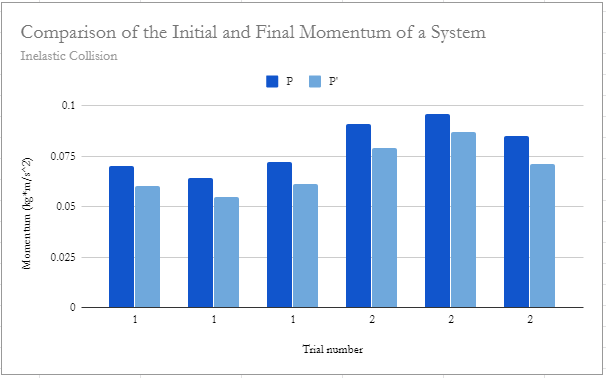
\includegraphics[width = 1 \columnwidth]{fig4.PNG}
    \caption{A plot comparing the initial and final momentum of a system after an inelastic collision.}
    \label{fig:1}
\end{figure}
Figure \ref{fig:1} shows a bar chart which highlights the difference between the initial momentum of a system, 
denoted $\vec{p}$ and marked in dark blue and the final momentum $\vec{p}\,'$ marked in light blue. In both Figure \ref{fig:1} and Figure \ref{fig:2}, 
momentum was measured in $\frac{kg}{m\cdot s^2}$. Figure \ref{fig:1}
highlights the differences between the initial and final momentum of the system, notably that there is relatively none. 
Since there are many sources of error as will be described in the following section, the two bars are not equivalent, but close. 
On average, the height of the bars (or difference in momentum) for trial 1 differ by $15.68\%$, while the height of the bars
in trial 2 differ by about $14.74\%$, a reasonable percent error for the data.
\begin{figure}
    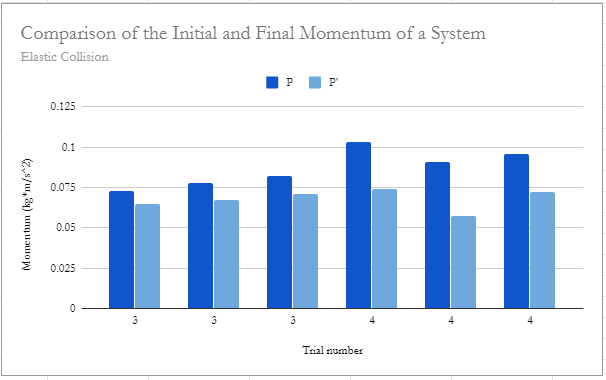
\includegraphics[width = 1 \columnwidth]{fig5.PNG}
    \caption{A plot comparing the initial and final momentum of a system after an elastic collision.}
    \label{fig:2}
\end{figure}

Similarly, let us turn our attention to Figure \ref{fig:2}. Figure two details the differences between the initial and final momentum
after an elastic collision. It is marked the same way as Figure \ref{fig:1}, and so we will gloss over the details, with the important
takeway being that the difference between the two bars is still quite small, with an average percent error for trial 3 being
$13.71\%$ and $39.97\%$ for trial 4. A discussion of the reasons for the error in trial 4 will follow in the following section. 
\subsection*{Conservation of Kinetic Energy}
\begin{figure}
    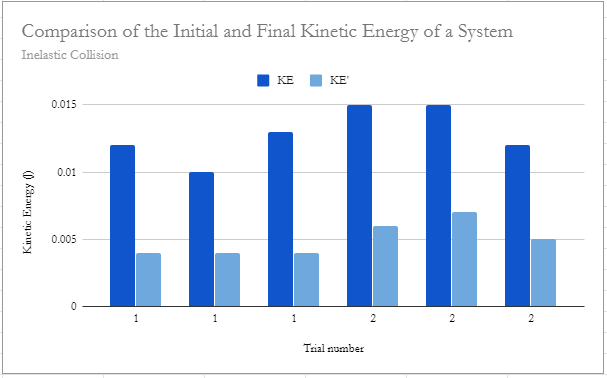
\includegraphics[width = 1 \columnwidth]{fig6.PNG}
    \caption{A plot comparing the initial and final kinetic energy of a system after an inelastic collision.}
    \label{fig:3}
\end{figure}
Observe Figure \ref{fig:3}, which is a bar chart highlighting the difference between the initial and final kinetic energy of a system after an 
inelastic collision. Kinetic energy is measured in $J$ (joules) in both Figure \ref{fig:3} and Figure \ref{fig:4}.
Our first deviation from the expected begins here: the difference in the height of the bars, representing the difference in kinetic energy before 
and after an inelastic collision, is quite massive. This means that kinetic energy is not conserved after an inelastic collision, supporting a fact we already knew.
To demonstrate this fact numerically, the average percent error for trial 1 was $97.20\%$, and the average percent error for trial 2 was
$76.25\%$. In this particular case, the error was the difference of these percent error values from $100\%$.

We know that elastic collisions conserve kinetic energy, and this can seen
from the bar chart for Figure \ref{fig:4}: similar to Figure \ref{fig:1} and Figure \ref{fig:2}, 
the difference in heights of the bars are low, meaning that kinetic energy is conserved.
Numerically, the average percent difference for trial 3 was $28.48\%$, while the average percent difference for trial 4 was
$27.43\%$.
\begin{figure}
    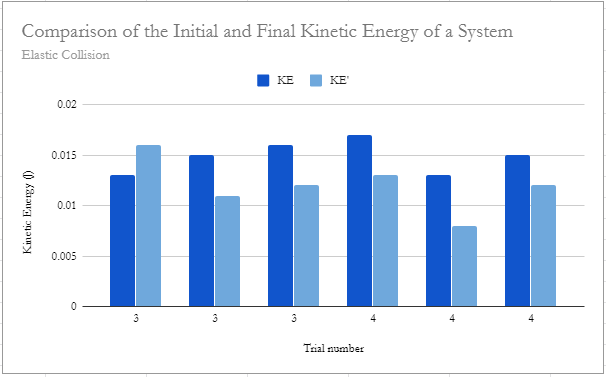
\includegraphics[width = 1 \columnwidth]{fig7.PNG}
    \caption{A plot comparing the initial and final kinetic energy of a system after an inelastic collision.}
    \label{fig:4}
\end{figure}
\section{Discussion of Results and Error Analysis}
The purpose of this experiment was to demonstrate the conservation of momentum and the conservation of kinetic energy for
inelastic and elastic collisions. As stated above, in the case of momentum, the average percent differences were
$15.68\%$ and $14.74\%$ for trials 1 and 2 which only differed in the mass of the object, and the average percent differences for
trials 3 and 4 were $13.71\%$ and $39.97\%$ respectively, which not only differed in mass between the trials but also had a different collision type, 
namely these collisions were elastic. The difference of these values from $0\%$ is the error in this experiment. Similaryl, in the case of 
kinetic energy, the average percent differences for trials 1 and 2 were $97.20\%$ and $76.25\%$. Since kinetic energy is not conserved
during an inelastic collision, in this case the error of the experiment was the distance from these values and $100\&$ error. Finally, 
the average percent difference for trials 3 and 4 were $28.48\%$ and $27.43\%$ respectively, with the error being the distance of these values from $0\%$.

As a discussion of error analysis, there are several possible sources of error from this experiment. In the case of our particular setup, the track
was not level with the floor, possibly due to the fact that the floor of the building itself was not level with the ground. In any case, our gliders would drift
downward even when parallel with the "floor" of the lab room, showing that the force of gravity acted to imbalance the position of the gliders even in a frictionless environment.
This was probably the main source of error for this experiment for us. However the results are not horrible, and so our conclusion still holds. Another possible source of
error would be the accuracy of the photogates and how far back we would hold the glider against the rubber band during the trials, generating various
levels of potential energy which differed from trial to trial. These errors can be solved or improved by changing lab setups and possibly acquiring more sophisticated technology
that can measure speed to an extremely precise level, and automate the launching process to ensure standardized results. 

In general, these results accomplish the goal of this experiment. They show that during an inelastic collision, only momentum is conserved,
while in the case of an elastic collision, both momentum and kinetic energy are conserved. Finally, since momentum is conserved in both elastic 
and inelastic collisions, the law of conservation of momentum holds to be true. 


\section{Conclusion}
In conclusion, the results of this experiment fully support the theory behind it. We theorized that momentum would be conserved no matter the collision or system, and this
held to be true, the highest error being $39.97\%$ in the case of momentum, and the lowest being $13.71\%$. This can be seen from the percent differences of the initial and final momentum between the trials, listed in the section above. Similarly, 
we also theorized that kinetic energy would be conserved in the case of an elastic collision, and would not be conserved in the case of an inelastic collision, which held to be true. 
The highest error was $28.48\%$, while the lowest error was a whopping $2.80\% \,(100.00\% - 97.20\%)$.
The method is sufficiently precise, since it yielded relatively accurate data that fit in with the theory. Some ways error could be reduced 
include the methods mentioned in the section above: fixing our setup, obtaining extremely precise laboratory grade equipment, and eliminating human error. 
However, the experiment as is suffices, since the error is low and the results accurate. 

\end{document}